\documentclass[12pt]{article}
 
\usepackage[margin=1in]{geometry} 
\usepackage{amsmath,amsthm,amssymb,outlines}
\usepackage{graphicx}
\usepackage{tikzsymbols}
\newenvironment{statement}[2][Statement]{\begin{trivlist}
\item[\hskip \labelsep {\bfseries #1}\hskip \labelsep {\bfseries #2.}]}{\end{trivlist}}
\newcommand\restr[2]{{% we make the whole thing an ordinary symbol
  \left.\kern-\nulldelimiterspace % automatically resize the bar with \right
  #1 % the function
  \littletaller % pretend it's a little taller at normal size
  \right|_{#2} % this is the delimiter
  }}

\begin{document}
 
\title{Algebraic Topology Homework 2} 
\maketitle

\begin{statement}[Exercise]{1}
    Describe a CW complex structure on $\mathbb{C}P^2 \times \mathbb{R}P^2$ and $\Sigma T^2$.
\end{statement}
\begin{proof}
    For $\mathbb{C}P^2 \times \mathbb{R}P^2$, we know that $\mathbb{R}P^2$ consists of 1 0-cell, 1 1-cell, and 1 2-cell. Similarly, for $\mathbb{C}P^2$, it consists of 1 1-cell, 1 2-cell, and 1 4-cell. Thus the product of these spaces consists of 1 0-cell, 1 1-cell, 2 2-cell, 1 3-cell, 2 4-cell, 1 5-cell, and 1 6-cell. Visually, we're finding the product of a sphere and a 4th dimensional shape.
    \par For $\Sigma T^2$, first note that $T^2 = S^1 \times S^1$, the torus. In Hatcher, it is stated that $\Sigma X = X \wedge S^1$, so in our case, $\Sigma (S^1 \times S^1) = (S^1 \times S^1) \wedge S^1$. Also in Hatcher, $ X \wedge Y = X \times Y / X \vee Y$. So finally, we have $ (S^1 \times S^1) \times S^1 / (S^1 \times S^1) \vee S^1$. Visually, we can imagine this as a torus crossed with $S^1$ quotient by a torus touching a circle. Regarding cell complexes, we have $(e^0 \cup e^1 \cup e^1 \cup e^1 \cup e^2 \cup e^2 \cup e^2 \cup e^3) / (e^0 \cup e^0 \cup e^1 \cup e^1 \cup e^1 \cup e^2)$. Thus the reduced suspension of a torus has the CW structure of 1 1-cell, 2 2-cells, and 1 3-cell.
\end{proof}

\begin{statement}[Exercise]{2}
    Let $X_n$ be the topological space obtained by identifying $n > 1$ points on $S^2$ to a single point. Describe a CW decomposition of $X_n$.
\end{statement}
\begin{proof}
    When you identify a point with a singular point, you're pinching the $S^2$ sphere at that singular point, and it creates a "loop" from where the point originally was to the singular point. This occurs for every point identified, so that there are $n-1$ loops (or $S^1$'s) added to the space. Note that we need loops, because if we were to do lines, some lines could intersect. Thus we can say $X_n = S^2 \vee \bigvee_{i=1}^{n-1} S^1$, which is just stating that $X_n$ is a sphere with loops added that intersect at a single point (the singular point). When considering CW decomposition, the $S^2$ has 1 0-cell and 1 2-cell, while each $S^1$ has a 0-cell and a 1-cell. However, the singular point can be made the 0-cell for the $S^2$ and the $S^1$'s, so in total there is 1 0-cell, 1 2-cell, and $n-1$ 1-cells. 
\end{proof}

\begin{statement}[Exercise]{3}
    Hatcher Exercise 0.21: If $X$ is a connected Hausdorff space that is a union of a finite number of 2-spheres, any two of which intersect in at most one point, show that $X$ is homotopy equivalent to a wedge sum of $S^1$'s and $S^2$'s.
\end{statement}
\begin{proof}
    First, because the space is connected, we know that there aren't any disjoint 2-spheres. Then, we can imagine this space made up of $S^2$'s which intersect at most 1 point, and because there can't be any disjoint 2-spheres, they must all be in a row like this, or in a loop:
    \par 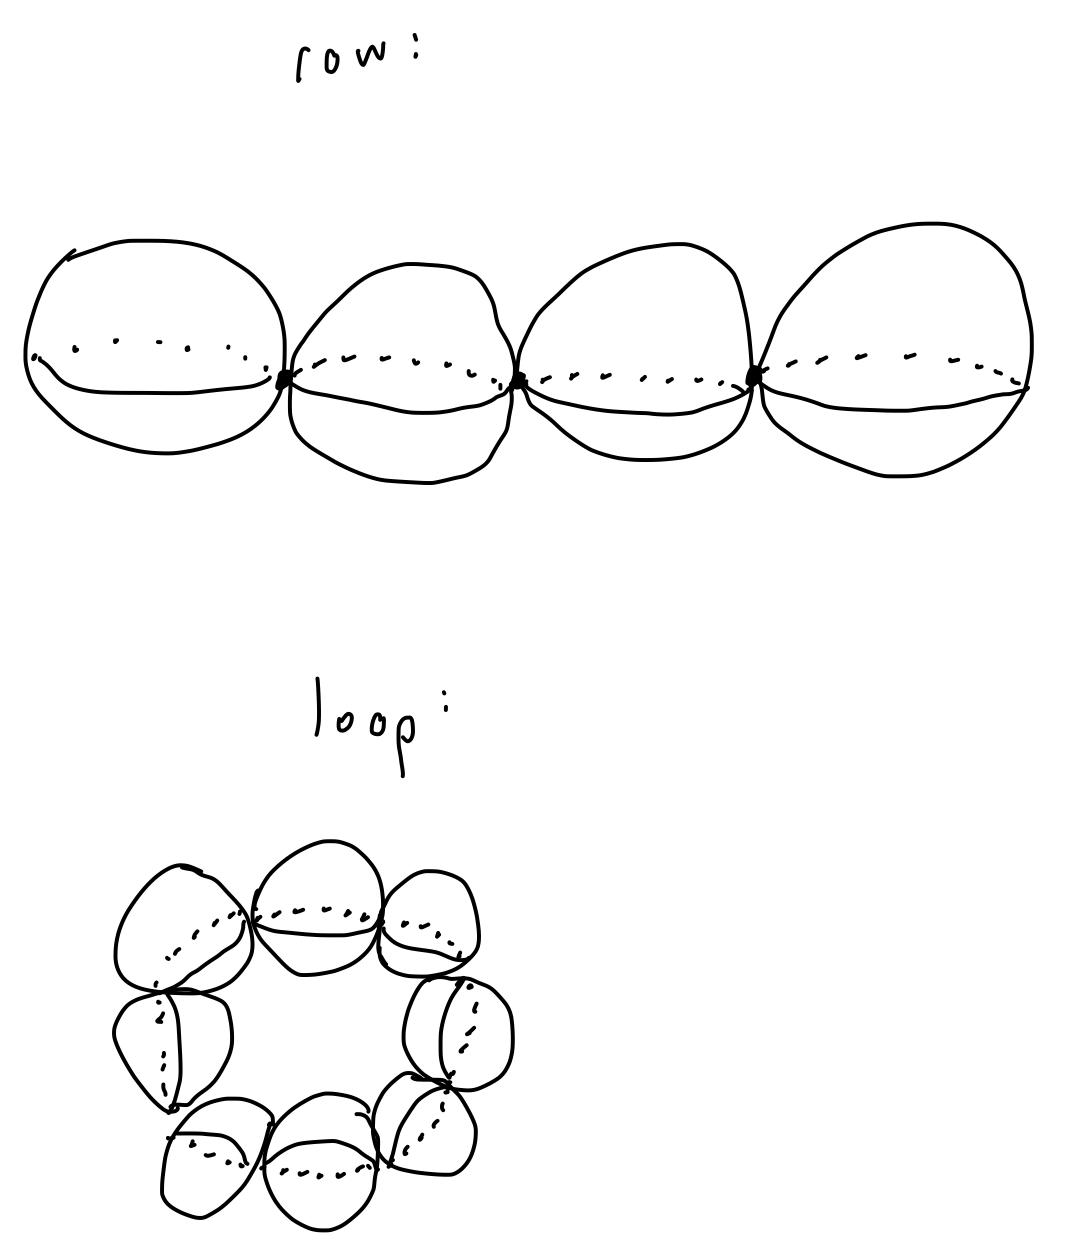
\includegraphics[scale=.2]{3-1.png}
    \par Either way, the intersection points between the spheres can be stretched into lines between them, like this:
    \par 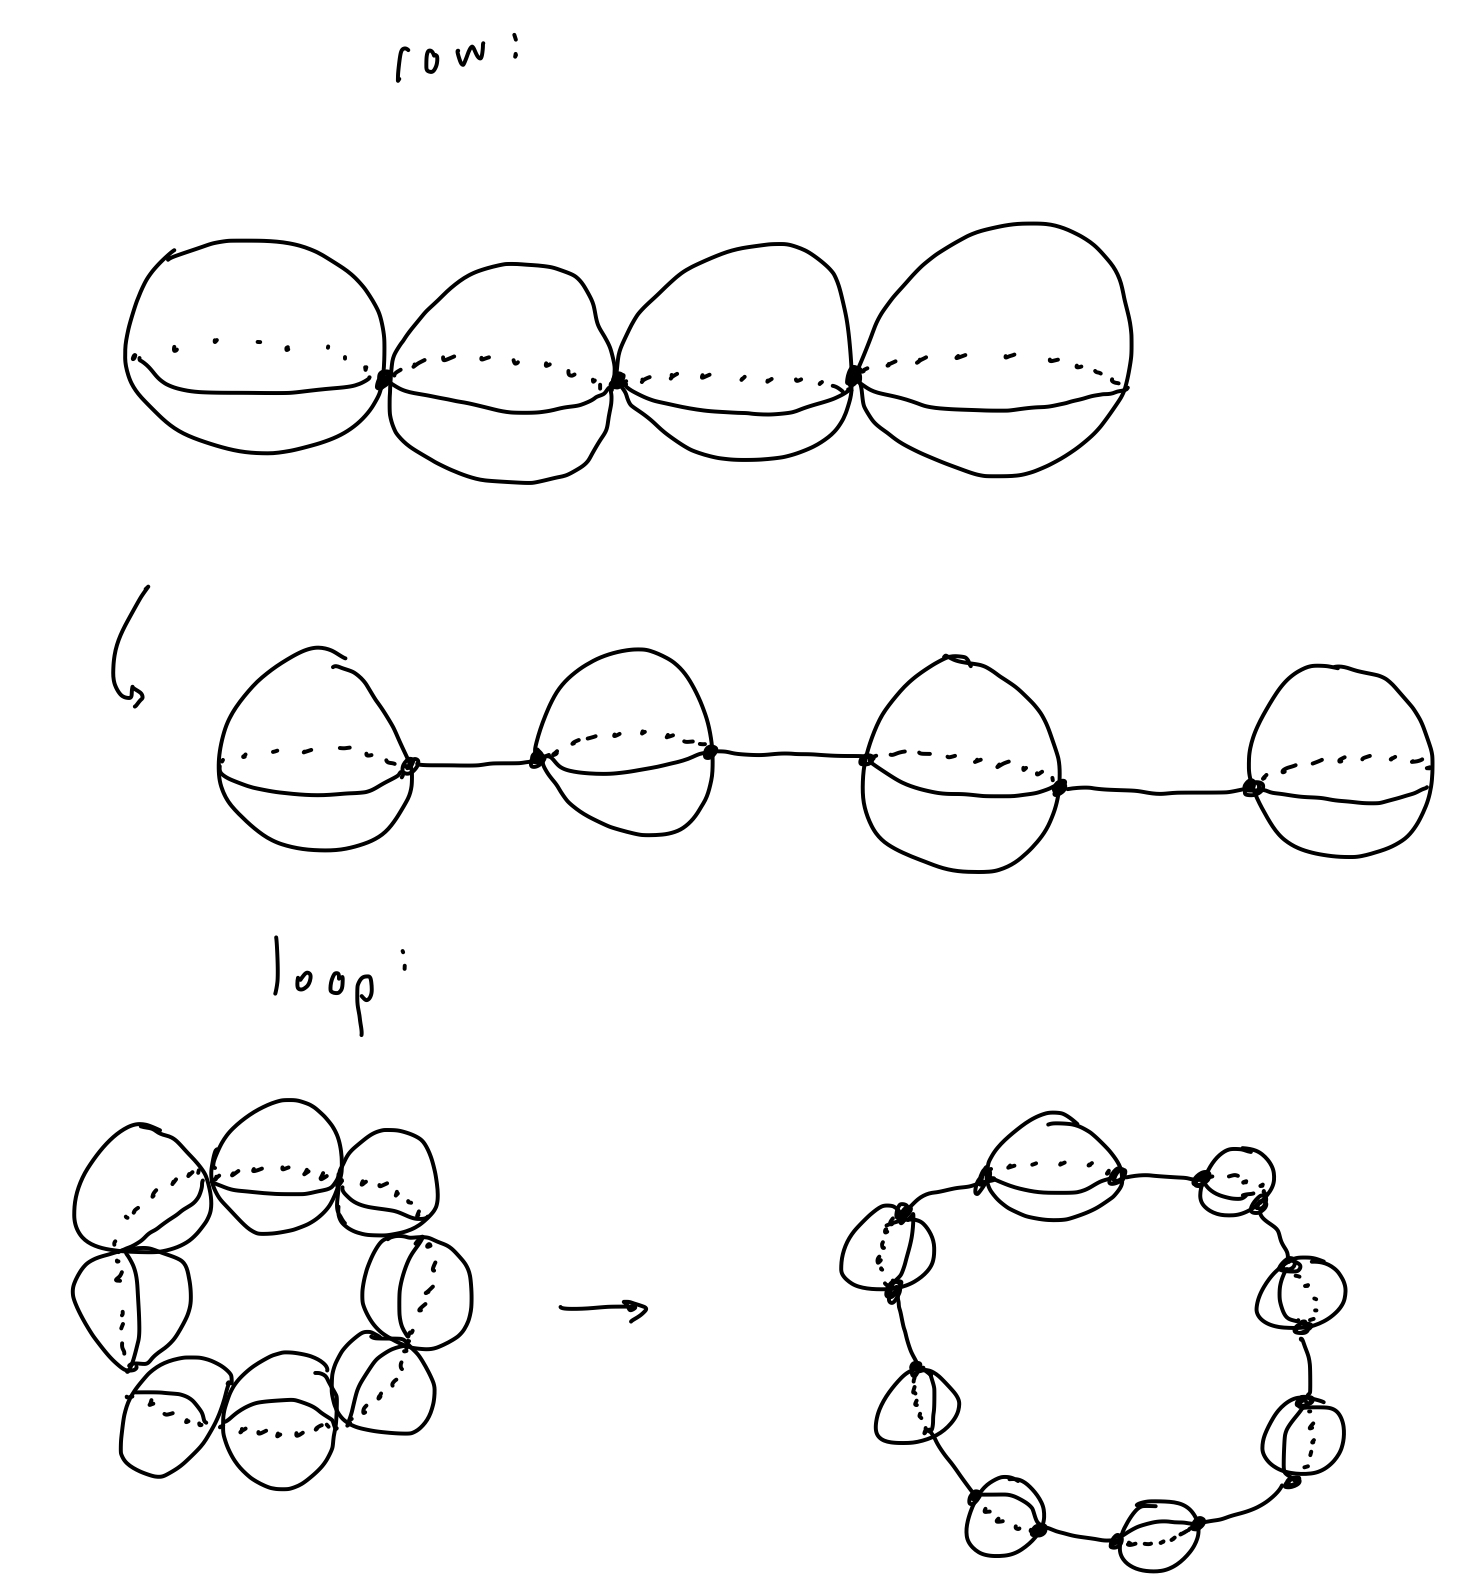
\includegraphics[scale=.2]{3-2.jpg}
    \par As you can see, the space $X$ can be stretched (and is therefore homotopically equivalent to) to be $\bigvee_{i=1}^{n-1} S^1 \vee \bigvee_{i=1}^{n} S^2$ where $n$ is the number of 2-sphere's in $X$. 
\end{proof}

\begin{statement}[Exercise]{4}
    Hatcher Exercise 0.25: If $X$ is a CW complex with components $X_{\alpha}$, show that the suspension $SX$ is homotopy equivalent to $Y \vee_{\alpha} SX_{\alpha}$ for some graph $Y$. In the case that $X$ is a finite graph, show that $SX$ is homotopy equivalent to a wedge sum of circles and 2-spheres. 
\end{statement}
\begin{proof}
    If $X$ is a finite graph, the suspension $SX$ is just taking all the vertices in the graph and connecting them to a point "above" and "below" the graph. This results in something like this: 
    \par 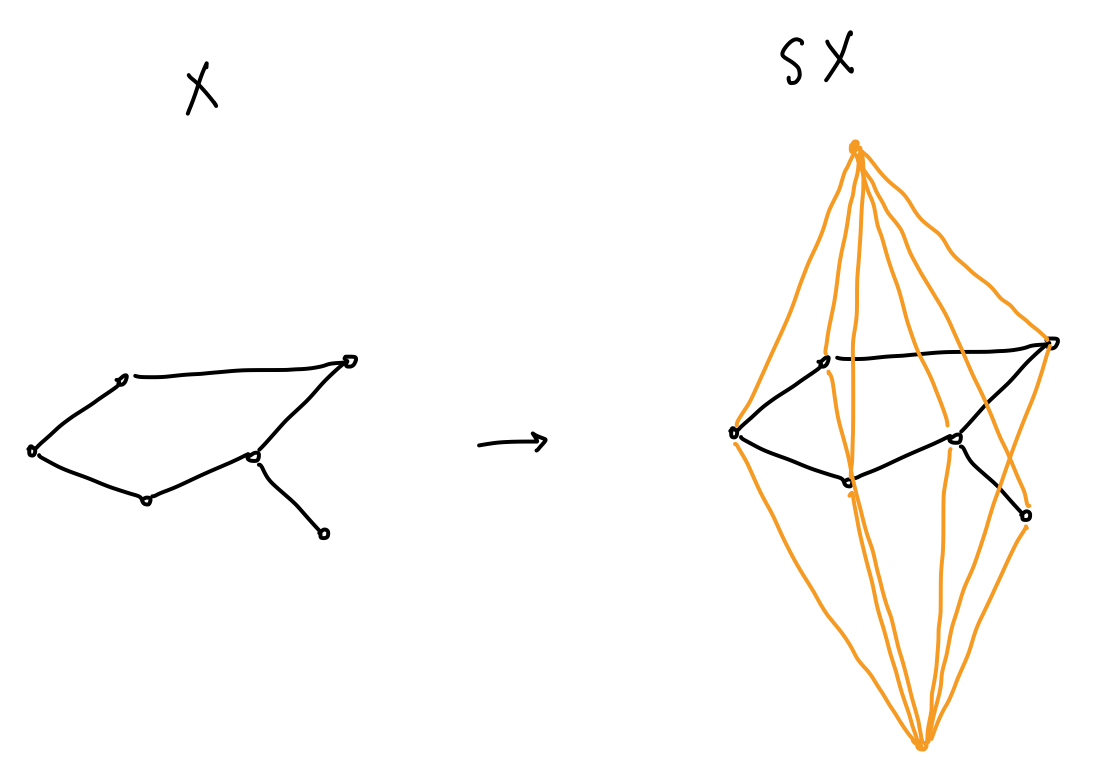
\includegraphics[scale=.2]{4-1.png}
    \par Note that when you have a closed loop in a graph, when you do the suspension it results in a sphere, and when there is a non-loop, it just creates circles:
    \par 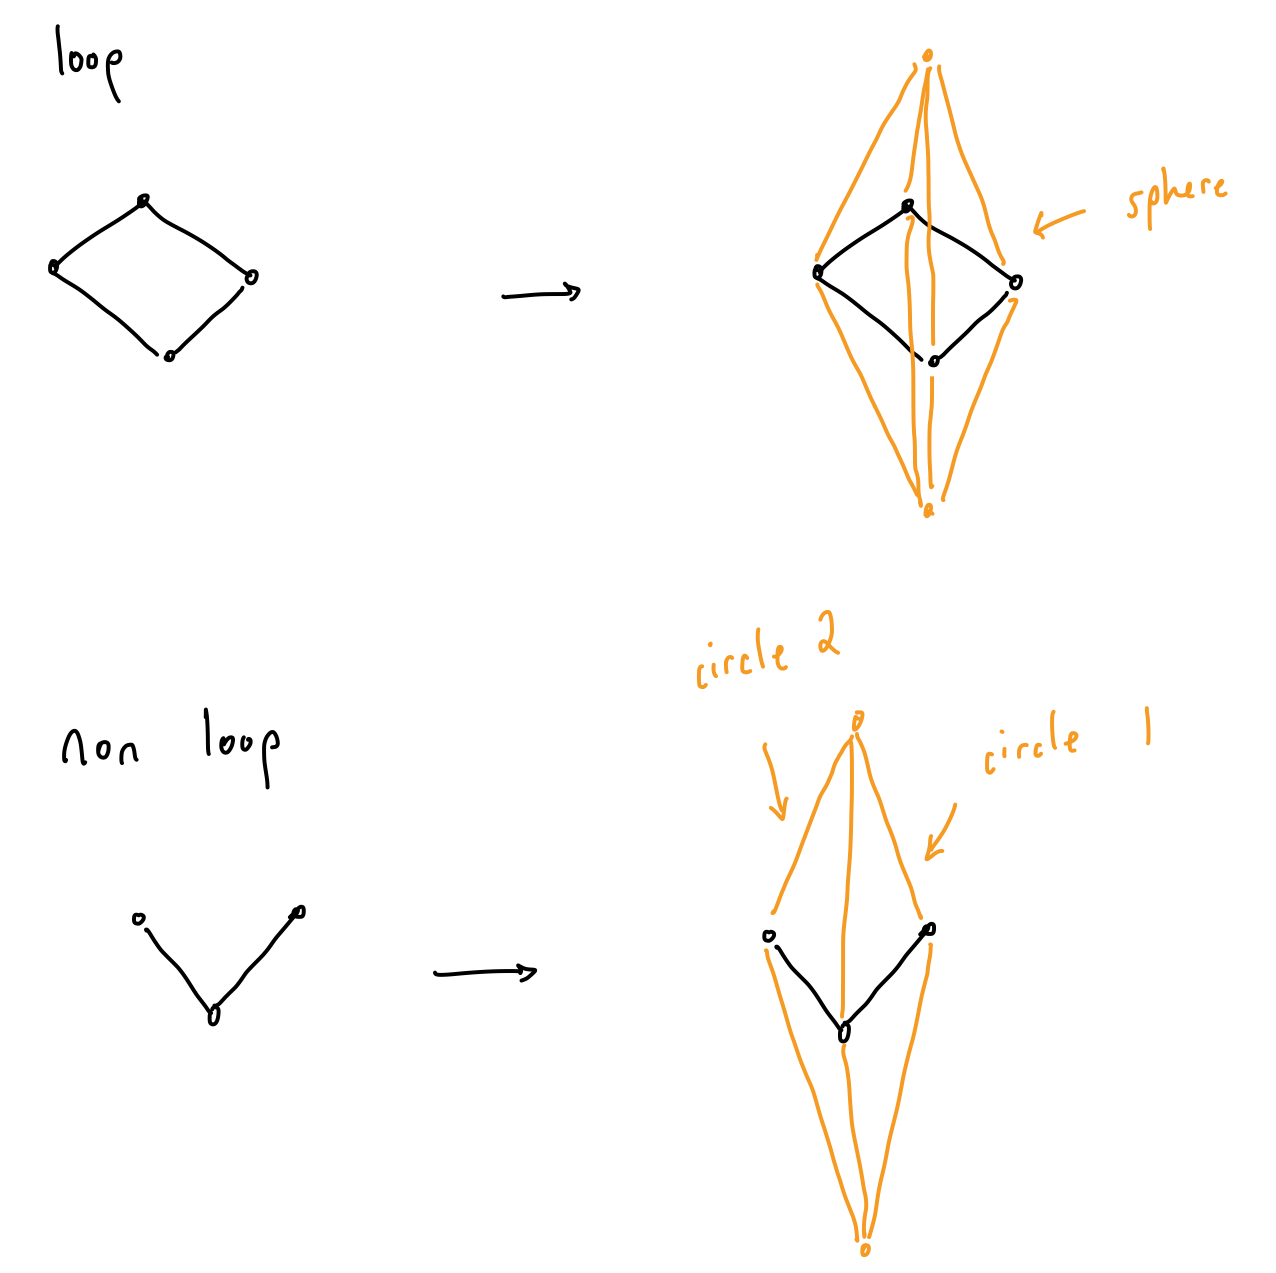
\includegraphics[scale=.2]{4-2.png}
    \par Because everything in a graph is either a loop or a nonloop, this accounts for what makes up any graph $X$. Thus if $X$ is a graph, $SX$ is just a wedge sum of spheres and circles. 
\end{proof}

\end{document}
